\section{Software Design og Implementering}

I projektet er det valgt at programmere i C++ frem for C. På microcontrolleren fås den store fordel at koden kan opbygges i klasser frem for frie funktioner. ATMega32 microcontrolleren er valgt, pga. kendskab til netop denne via MSYS på første semester. Encapsulation fra C++ giver bedre sikkerhed for fejl, da det har været muligt, at tilgå member-data via mutator/accessor metoder. 

Det første tiltag under designfasen var angående, hvad design dokumentet skulle indeholde. Der blev udarbejde nogle klassebeskrivelser udfra applikationsmodelen på side \pageref{P-fig:PC_klasse} i dokumentationen. Da klassebeskrivelserne var lavet, blev der skrevet metodebeskrivelser til dem, så det var klart hvilke funktionaliter, returværdier og parameter lister metoderne skulle indeholde.
Under forløbet blev arbejdet opdelt, og uddelegeret under en modificeret version af Scrum.

Derefter blev proktokollen mellem boundary klasser udformet, så ingen misforståelser ville ske for de personer, som skulle implementere hver sin del af domæneområdet. Protokollen blev holdt så simpel som muligt, da fejl over kommunikationsmediet skulle minimeres.

\subsection{PC Domæne}

\begin{figure}[h]
	\centering 
	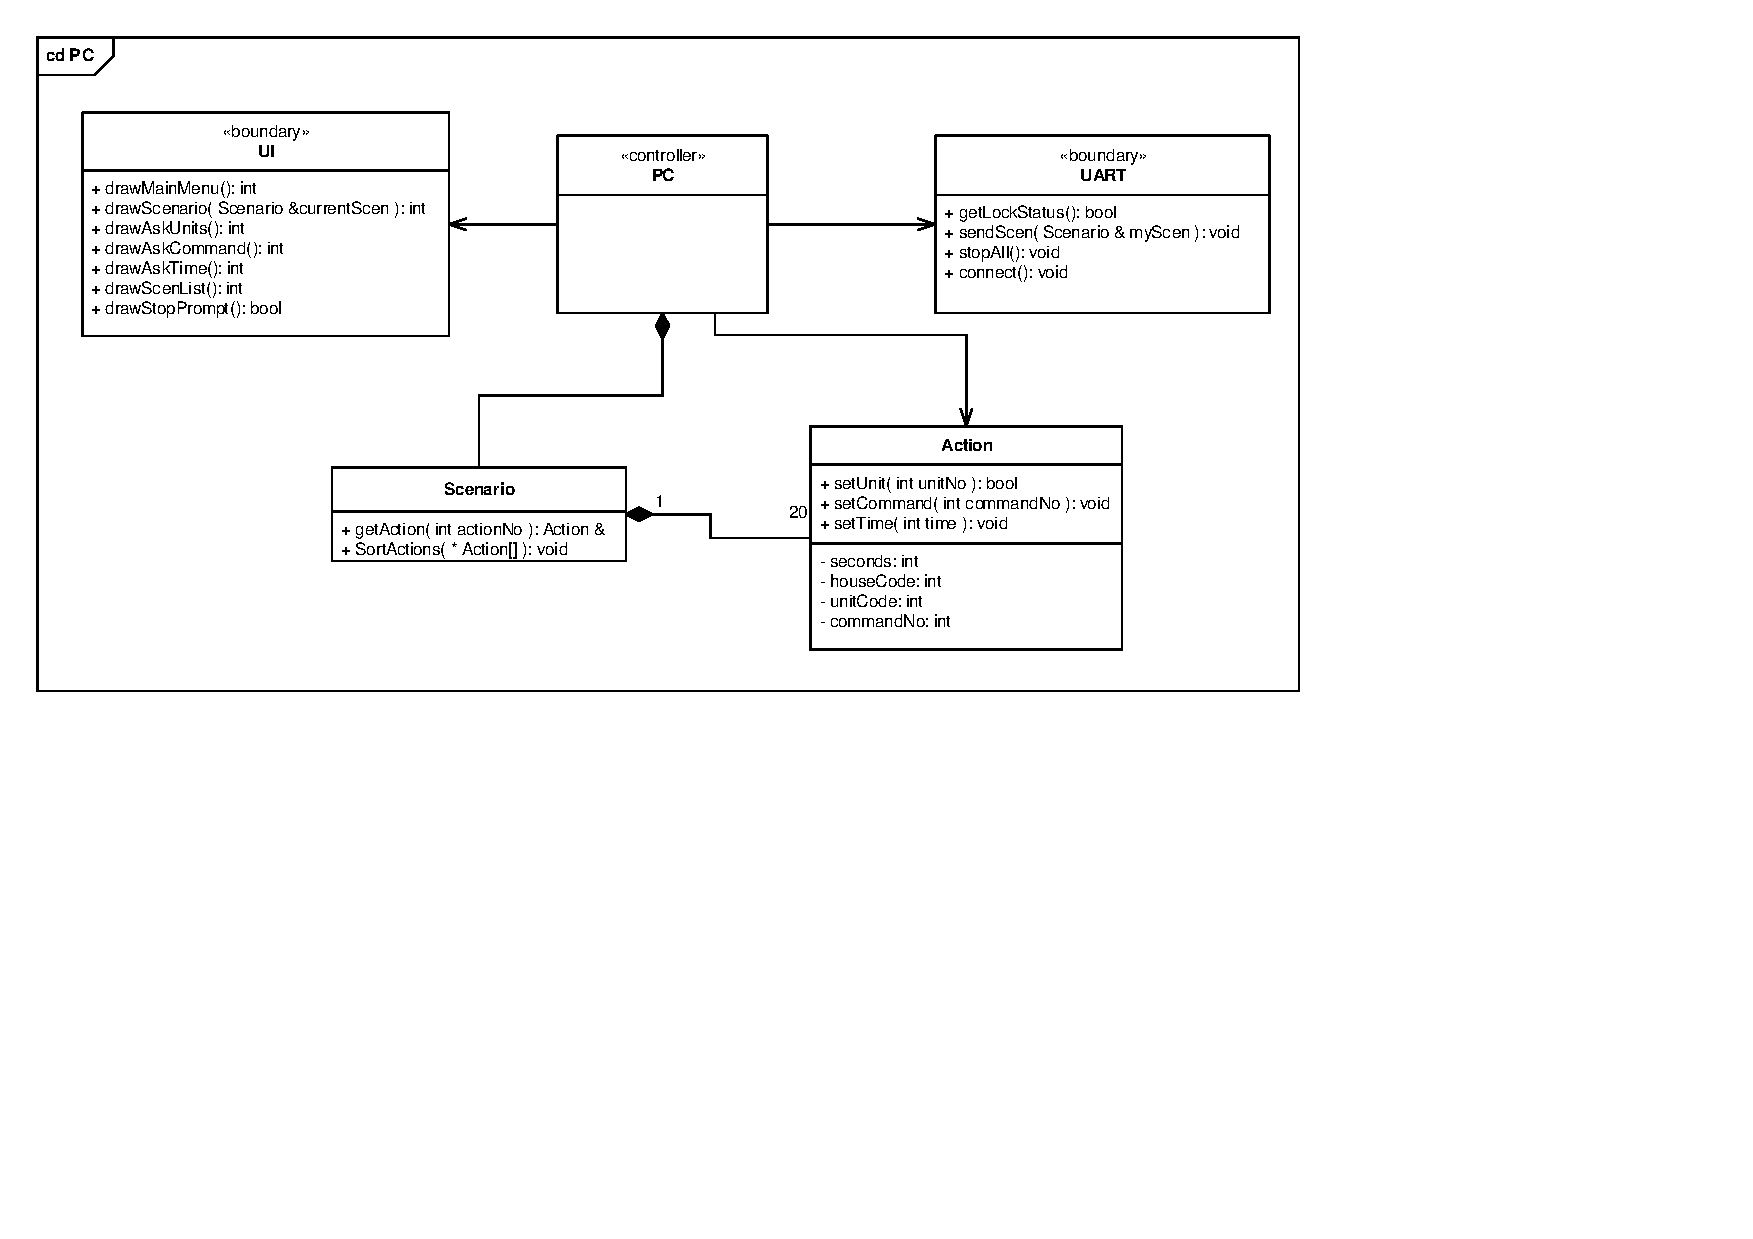
\includegraphics[width=\textwidth,trim=17 260 200 15, clip=true]{Projektbeskrivelse/Design_SW/diagrammer/PC_KlasseDiagram.pdf}
	\caption{Klassediagram for PC domænet}
\end{figure}

\texttt{PC Main} er ikke en klasse, men derimod den proces der sker når programmet eksekveres. Den har til opgave at kalde de rigtige metoder fra UI-klassen og gemme de data, den får fra brugeren ind i det korrekte actions objekt.
PC Main har også til opgave at transmittere data fra Scenariet, fra Scenario objektet, over til transmitteren ved brug af UART klassen.

\texttt{UART}-klassen har funktionaliteten til at sende strenge af data over til transmitteren igennem et RS232 kabel. Den har også mulighed for at kunne modtage respons fra transmitteren, når den skal have status på kodelåsen, som er tilknyttet transmitteren. UART'en oversætter den hentede data fra actions objekterne, så de følger protokollen for UART transmitteringen.
UART'en gør brug af et open source RS-232 biblioteket \cite{lib:UART}, og bruger dens funktioner til at forbinde til en gyldig COM-port, og sende og modtage data.

\texttt{Scenario}-klassen bruges til at holde de 20 actions objekter i. Den kan bruges til at hente de enkelte aktioner ud til manipulation og udskrivning af aktionerne på skærmen.
Scenario-klassen har også en sorteringsfunktion til at sortere aktionerne efter tid, så den tidligste tid står øverst og seneste tid nederst.

\texttt{Action}-klassen er til lagering af data, vedrørende hvad der skal ske på systemet. Ved brug af get- og set-metoder kan der manipuleres med dataen, så de kan tilpasses til den ønskede handling.

\texttt{UI}-klassen bruges til at have brugerinterfacet med på skærmen. Hver metode i klassen har til formål at fjerne tidligere indhold på skærmen, og tegne den nye menu. Efter menuen er på skærmen, har hver metode til formål at validere det input der kommer fra brugeren, og returnere informationer når gyldigt input registreres. UI klassen er den eneste mulighed brugeren har for at styre systemet på.

  
\subsection{Transmitter Domæne}

\begin{figure}[h]
	\centering \resizebox{\textwidth}{!}{
	\includegraphics[scale=0.5,trim=17 200 180 15, clip=true]{Projektbeskrivelse/Design_SW/diagrammer/Transmitter_KlasseDiagram.pdf}}
	\caption{Klassediagram for transmitter domænet}
\end{figure}

\texttt{Transmitter}-klassen holder styr på, at de forskellige klasser kan snakke sammen. Den indeholder også alle de actions, som bliver overført via UART'en.

\texttt{Codelock}-klassen tjekker, om koden er indtastet rigtigt på DE2 bordet.

\texttt{UART}-klassen kommunikerer med PC'en via UART, hvor der sendes informationer om status på codelock og der modtages scenarier fra PC'en. Her modtages 100 chars som svarer til 20 aktioner. Kommunikationsvejen er over RS232.

\texttt{Tx10}-klassen styrer alt kommunikation mellem transmitteren og receiverne, som foregår på el-nettet gennem X.10 protokolen. Timeren sørger for at sendes nøjagtigt i et milisekund.

\texttt{Action}-klassen holder styr på aktioner som skal køres på receiverne. Disse indeholder time, unit, command og house code så den ved hvor, de forskellige data skal sendes hen.

\texttt{Time}-klassen holder styr på tiden, så scenariet kan blive eksekveret til den ønskede tid. Timer1 bruges til at generere et interrupt hvert sekund, men det sendes kun videre til controlleren hver femte sekund for at være sikker på, at den kan nå at sende informationer over X.10 uden problemer. 

\subsection{Receiver Domæne}

\begin{figure}[h]
	\centering \resizebox{\textwidth}{!}{
	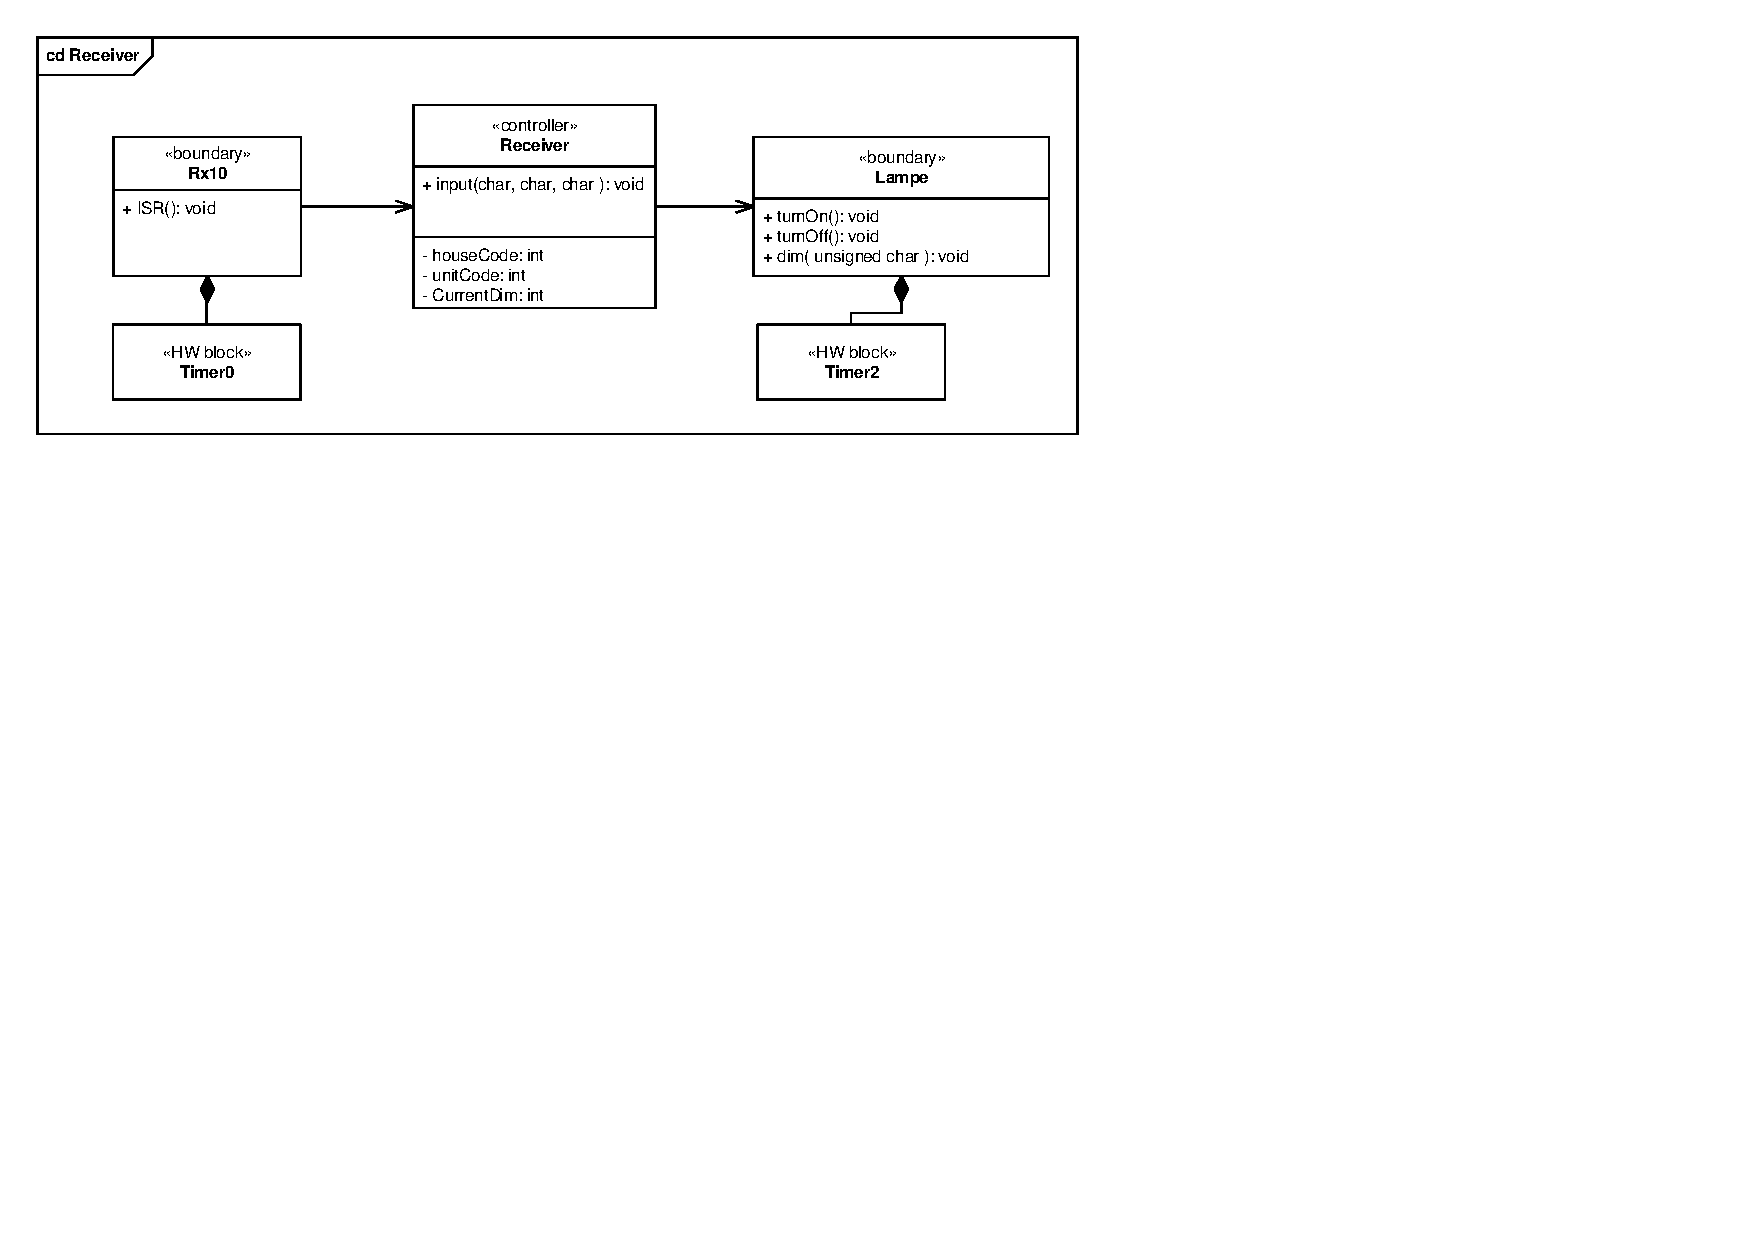
\includegraphics[scale=1,trim=17 380 320 18, clip=true]{Projektbeskrivelse/Design_SW/diagrammer/Receiver_KlasseDiagram.pdf}}
	\caption{Klassediagram for receiver domænet}
\end{figure}

\texttt{Rx10}-klassen er en boundary til Transmitter domænet, og har til opgave at modtage kommandoer fra X.10 nettet, samt formidle dem til receiver controller klassen.

\texttt{Timer0} er indbygget i ATmega32, og bruges af Rx10 klassen til at kontrollere for et 120kHz signal et halvt milisekund efter en nulgennemgang på 50Hz signalet.

\texttt{Receiver}-klassen manipulerer et Lampe objekt alt efter hvilken kommando der modtages.

\texttt{Lampe}-klassen styrer tænd, sluk og dim funktionaliteten.

\texttt{Timer2} bruges til at lave et variabelt PWM signal, der kan ændres af Lampe-klassen.


\subsection{Software Implementering}

Ved start af implementeringsfasen blev alle klasser skrevet ind på et Scrum-board, hvorefter hver udvikler kunne tage en opgave og gå i gang med at implementere den. Implementeringsfasen kørte som en iterativ procces, hvor softwareudvikleren først implementerede designbeskrivelsen og skrev modultest dertil. Dernæst blev klassen sendt til en delvis integrationstest, som er afhængig af dens funktionalitet. Se s. \pageref{P-TxUART} i dokumentationen.

Undervejs blev der fundet mangler og udnødvendige klasser i designbeskrivelsen. Ydermere skulle UART protokollen fra design revideres pga. fejl i modultesten. Fejlen var at værdien 'null' ikke kunne sendes med RS-232 biblioteket. Løsningen var at skifte fra '0-255' til '48-63', således at der kun er 16 brugbare værdier i hver sendt char istedet for 256. Skiftet resulteret i der nu skulle sendes 3 chars, istedet for 2 chars, til at overføre tiden for en enkelt aktion.

Der opstod problemer med at Rx10, fordi ''sladrehanks klassen'', se side \pageref{P-Rx} i dokumentation, var meget lang tid om at sende data ud af RS-232 porten. Problemet var at den ikke var interrupt baseret, og derfor hentede/sendte data hele tiden. 